\documentclass{beamer}
\usetheme[shownavsym]{AAUsimple}
\usefonttheme{structurebold}
%%%%%%%%%%%%%%%%%%%%%%%%%%%%%%%%%%
\usepackage[utf8]{inputenc}
\usepackage[dutch]{babel}
\usepackage[T1]{fontenc}
\usepackage{tikz}
\usepackage{hyperref}
\usepackage{microtype}
\usetikzlibrary{trees}
%%%%%%%%%%%%%%%%%%%%%%%%%%%%%%%%%%
% Gekleurde hyperlinks
\newcommand{\chref}[2]{%
	\href{#1}{{\usebeamercolor[bg]{AAUsidebar}#2}}%
}
\title[Hema compositie en hemapoïese]{Bloed  \& Anemie}

\date{\today}

\author[Edon Namani, et. al]
{%
	Edon Namani\\
	\href{mailto:e.namani@student.rug.nl}{{\tt e.namani@student.rug.nl}}
}

\institute[%
	Faculteit Gezondheidswetenschappen\\
	Rijksuniversiteit Groningen\\
	Nederland
]
{%
	Faculteit Gezondheidswetenschappen\\
	Rijksuniversiteit Groningen\\
	Nederland

}

\pgfdeclareimage[height=1.5cm]{titlepagelogo}{AAUgraphics/semper_invicta.pdf}
\titlegraphic{%
	\pgfuseimage{titlepagelogo}
}

\begin{document}
% Titel
{\aauwavesbg%
	\begin{frame}[plain,noframenumbering]
	\titlepage
\end{frame}}
%%%%%%%%%%%%%%%

%TOC
\begin{frame}{Agenda}{}
	\tableofcontents
\end{frame}
%%%%%%%%%%%%%%%

\section{Samenstelling van bloed}
\begin{frame}{Samenstelling}{Bloed} 
	\only<1>{%
		\begin{block}{Definitie}
		Bloed is een vorm van bindweefsel dat bestaat uit extracellulaire vloeistof bevattend "vormende elementen". Vormende elementen omvatten de leukocyten, erythrocyten en bloedplaatjes.
	\end{block}
}
	\only<2>{%
		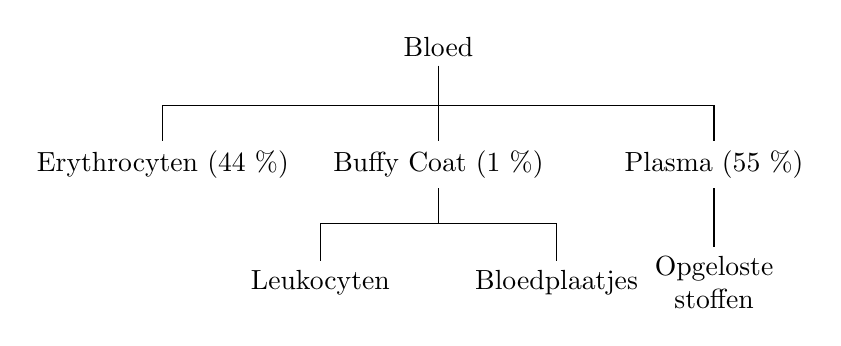
\begin{tikzpicture}[%
			level distance=1.5cm,
			level 1/.style={sibling distance=3.5cm},
			level 2/.style={sibling distance=3.0cm},
			every node/.style={align=center}
			]
			\node (1) {Bloed}
				[edge from parent fork down]
				child { node (2) {Erythrocyten (44 \%)}}
				child { node (3) {Buffy Coat (1 \%)}
					child { node (3sub1) {Leukocyten}}
					child { node (3sub2) {Bloedplaatjes}}
				}
				child { node (4) {Plasma (55 \%)}
						child { node (4sub1) {Opgeloste\\ stoffen}}
					};
		\end{tikzpicture}
}
\end{frame}
%%%%%%%%%%%%%%%

\section{Hemapoïese}
\begin{frame}{Hemapoïese}{Bloed}
	\begin{figure}
		\includegraphics[scale=.16]{./hemapoiese.png}
	\end{figure}
\end{frame}

{\aauwavesbg
\begin{frame}[plain,noframenumbering]
	\finalpage{Vragen?}
\end{frame}}
\end{document}
